\begin{figure}[htpb]
	\centering

\newcounter{y}
\setcounter{y}{0}

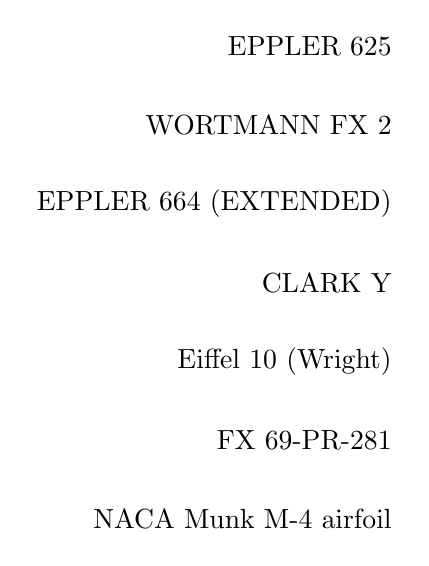
\begin{tikzpicture}
    \foreach \lbl / \fn in {EPPLER 625/e625.dat,
                            WORTMANN FX 2/fx2.dat,
                            EPPLER 664 (EXTENDED)/e664ex.dat,
                            CLARK Y/clarcy.dat,
                            Eiffel 10 (Wright)/eiffel10.dat,
                            FX 69-PR-281/fx69pr281.dat,
                            NACA Munk M-4 airfoil/m4.dat}{
        % Some profiles look better when using plot[smooth]
        \draw[yshift=-\arabic{y}cm,scale=3] node[left=0.5cm] {\lbl}
            plot file{tikz/data/\fn} -- cycle;
        \stepcounter{y}
    }  
\end{tikzpicture}
	
	\caption{Tragfl\"achenprofile\protect\footnotemark}
	\label{fig:airfoil_general}
\end{figure}